%!TEX root = ../Demo.tex
\chapter{照片展示}
\section{实物展示}
以下是我们的作品实物展示照片:

\begin{figure}[H]
  \centering
  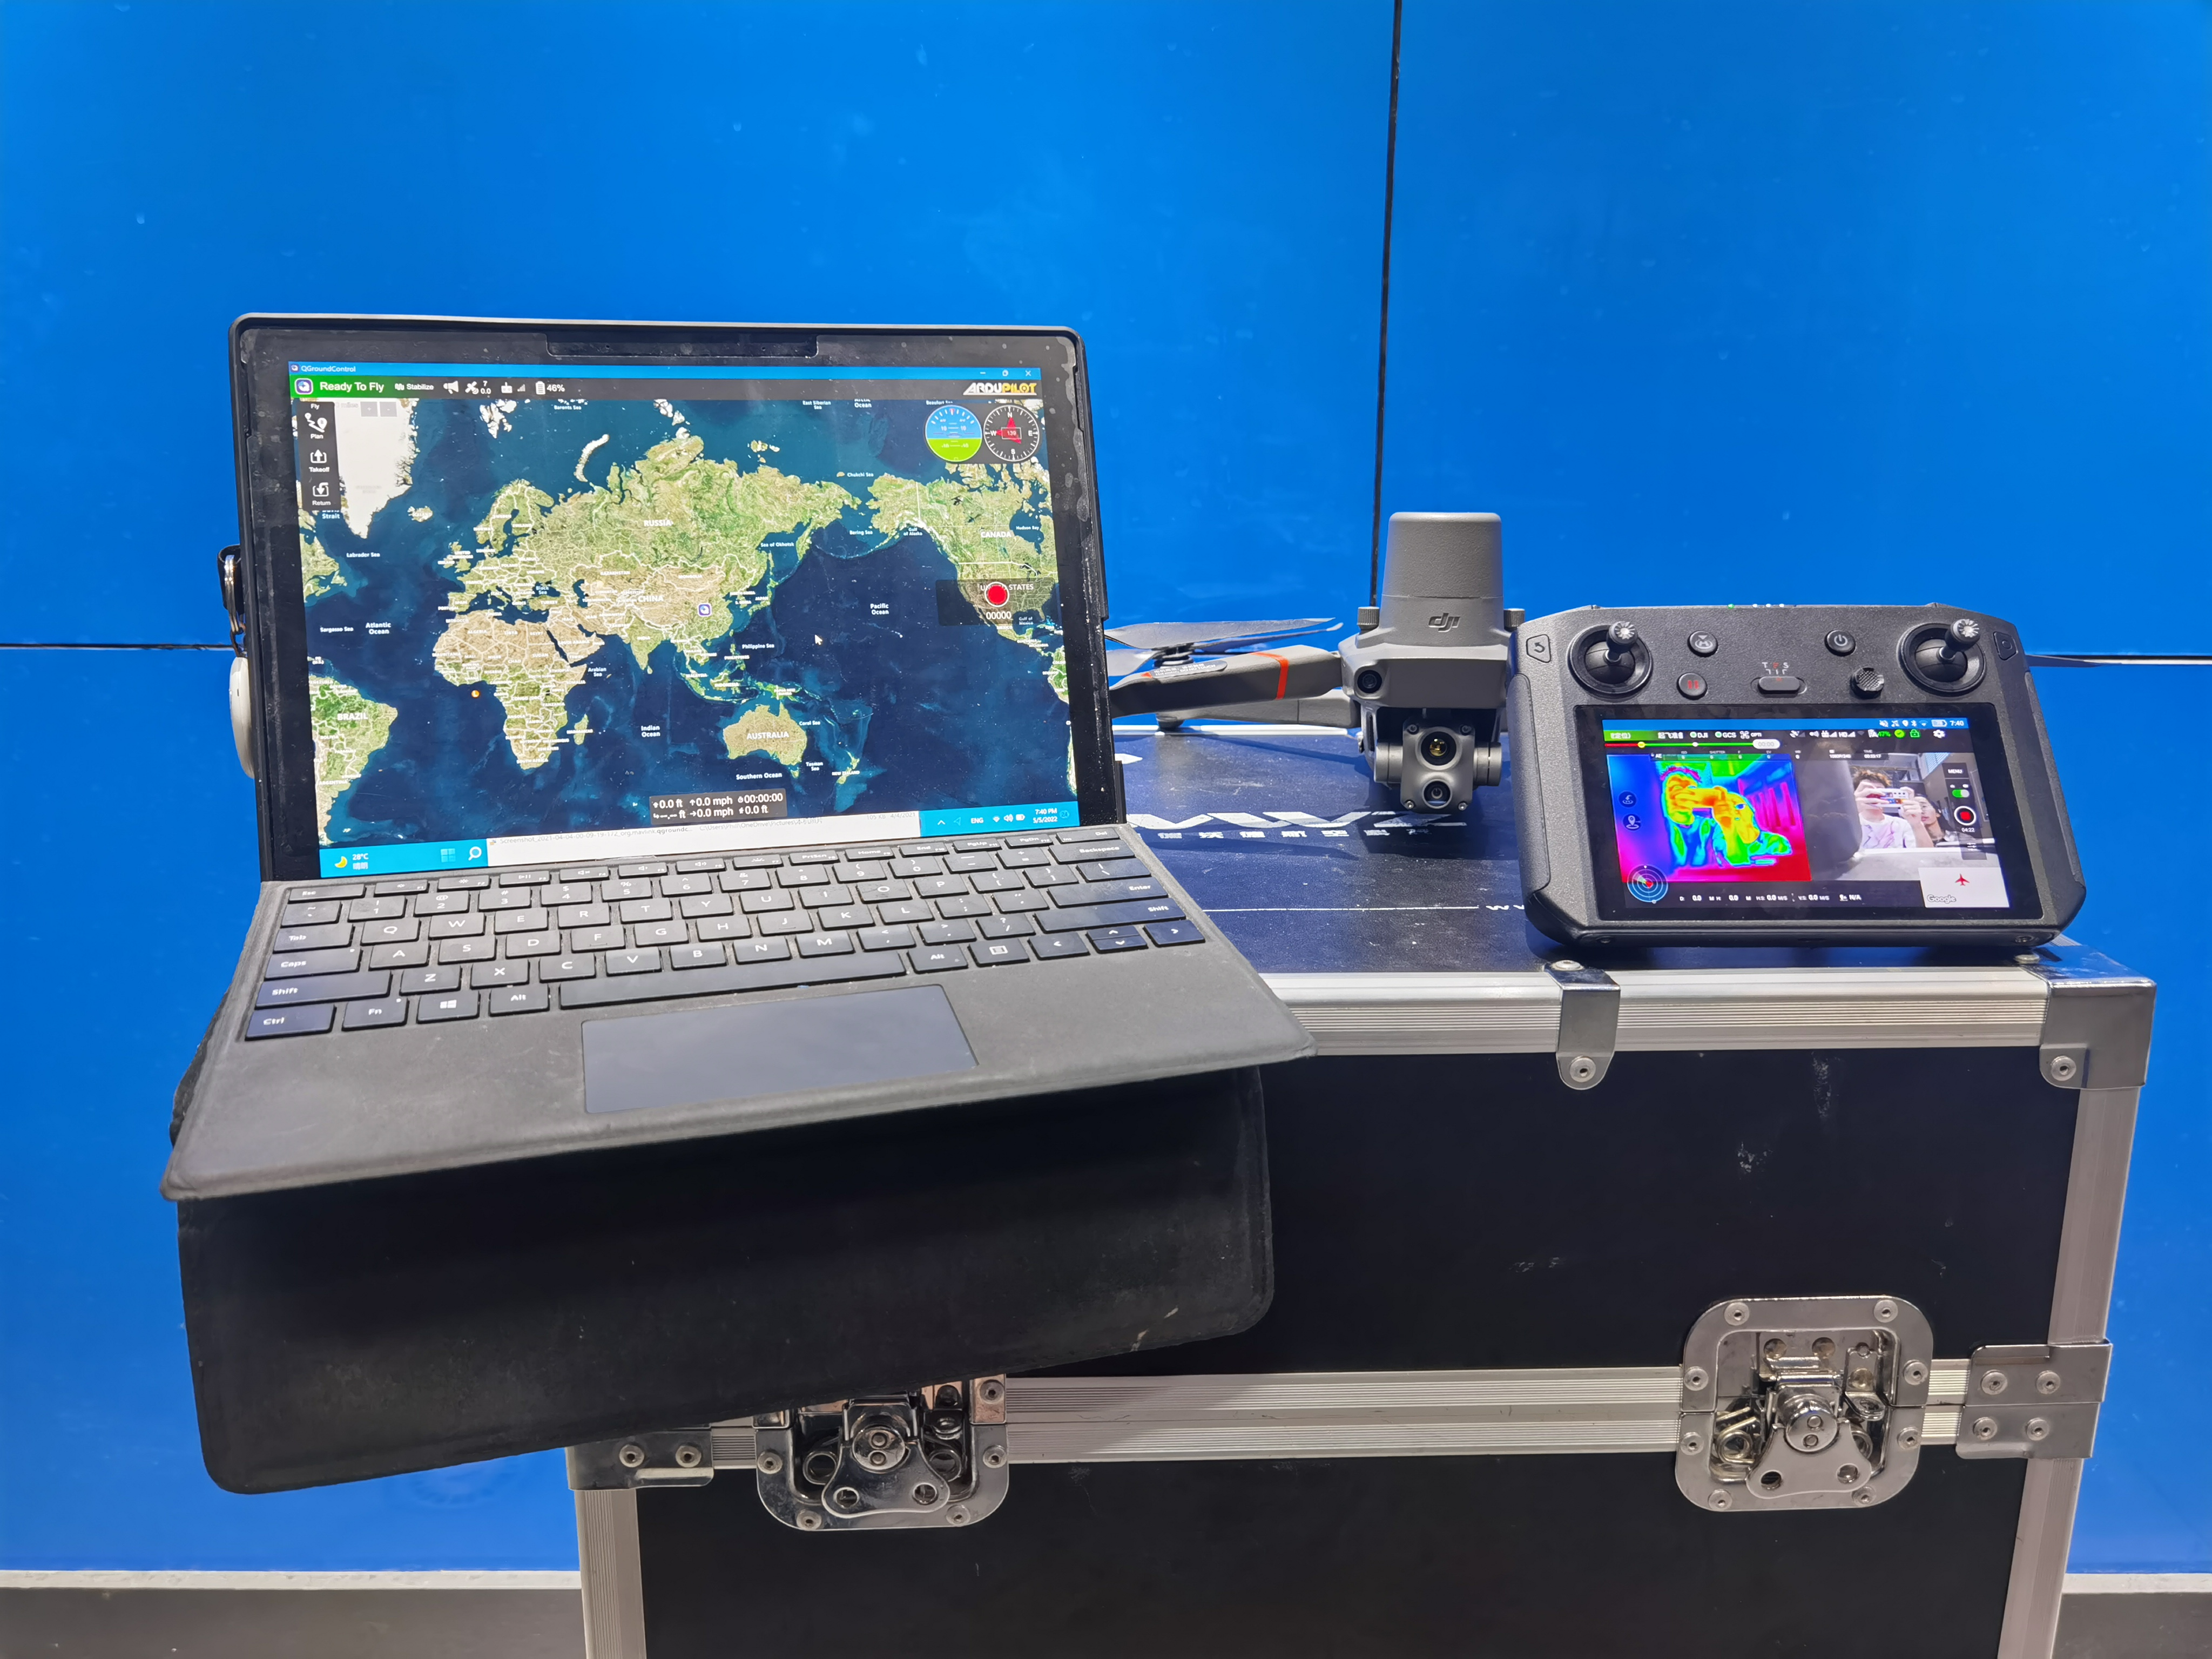
\includegraphics[width=0.8\linewidth]{./Figure/Real_Picture.jpg}
  \caption{作品实物展示照片}\label{Fig:append_img1}
\end{figure}

\section{效果测试}
效果测试照片(右下角小窗口内的是识别的降落板):

\begin{figure}[H]
  \centering
  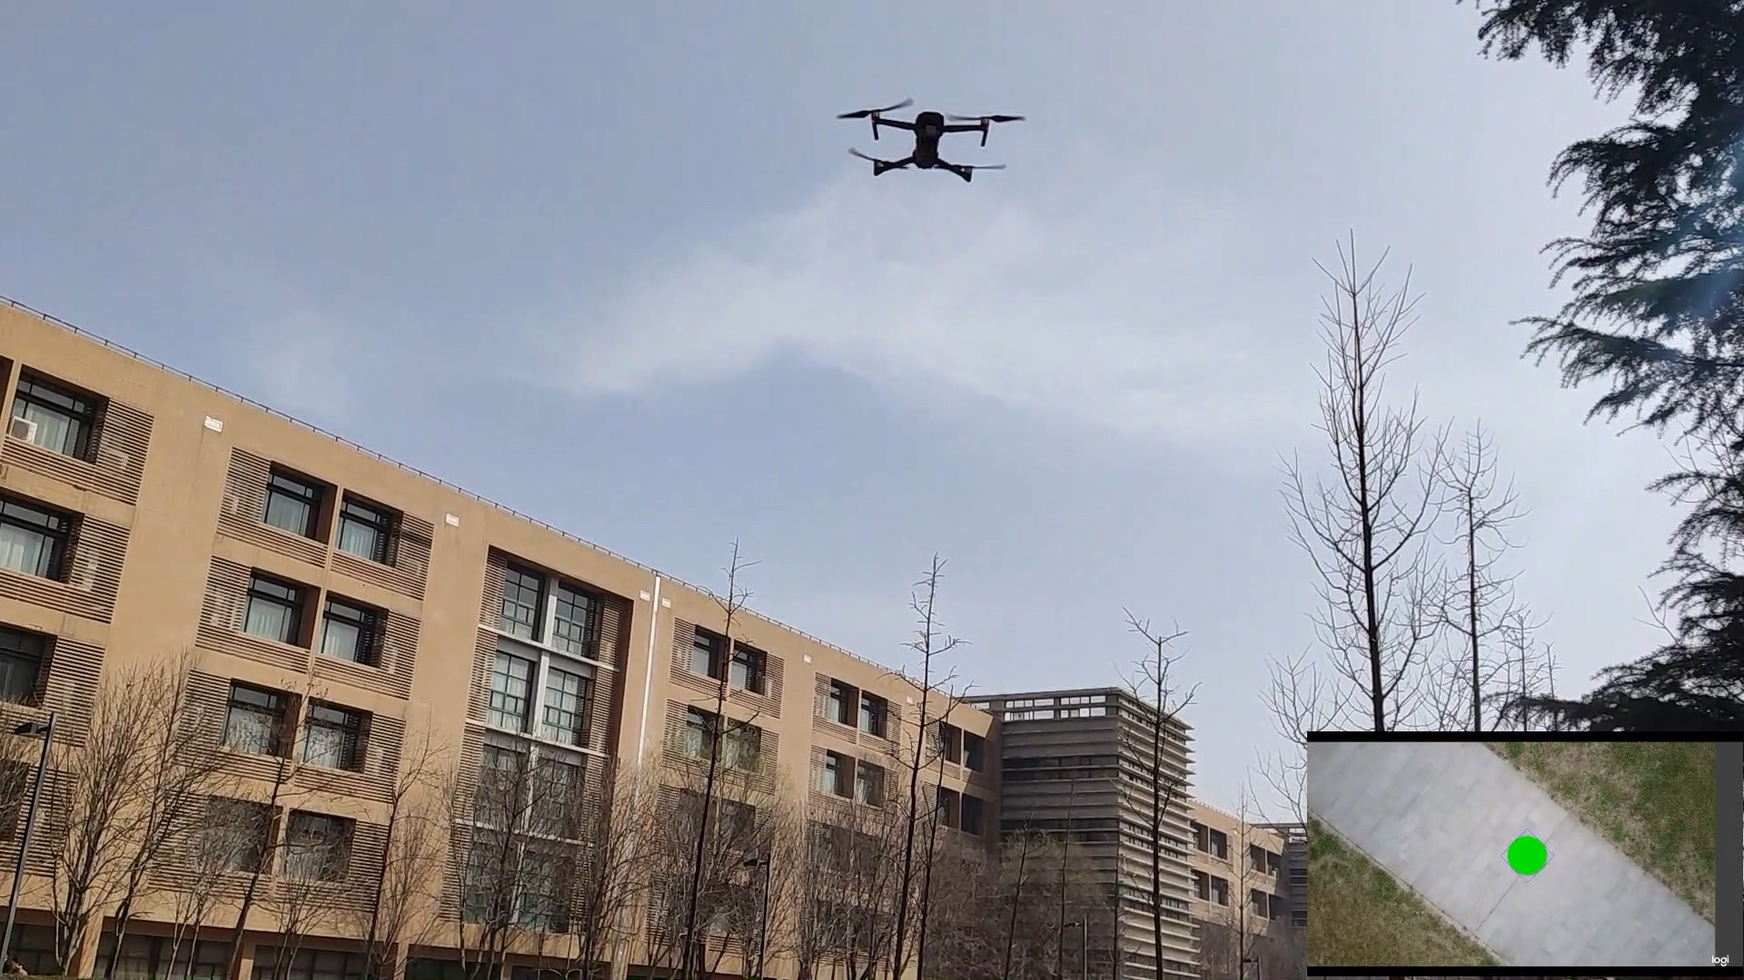
\includegraphics[width=0.8\linewidth]{./Figure/Landing_Real_Picture.jpg}
  \caption{作品实物展示照片}\label{Fig:append_img2}
\end{figure}

\section{APP软件截图}
APP启动、带屏遥控器设备识别界面:

\begin{figure}[H]
    \centering
    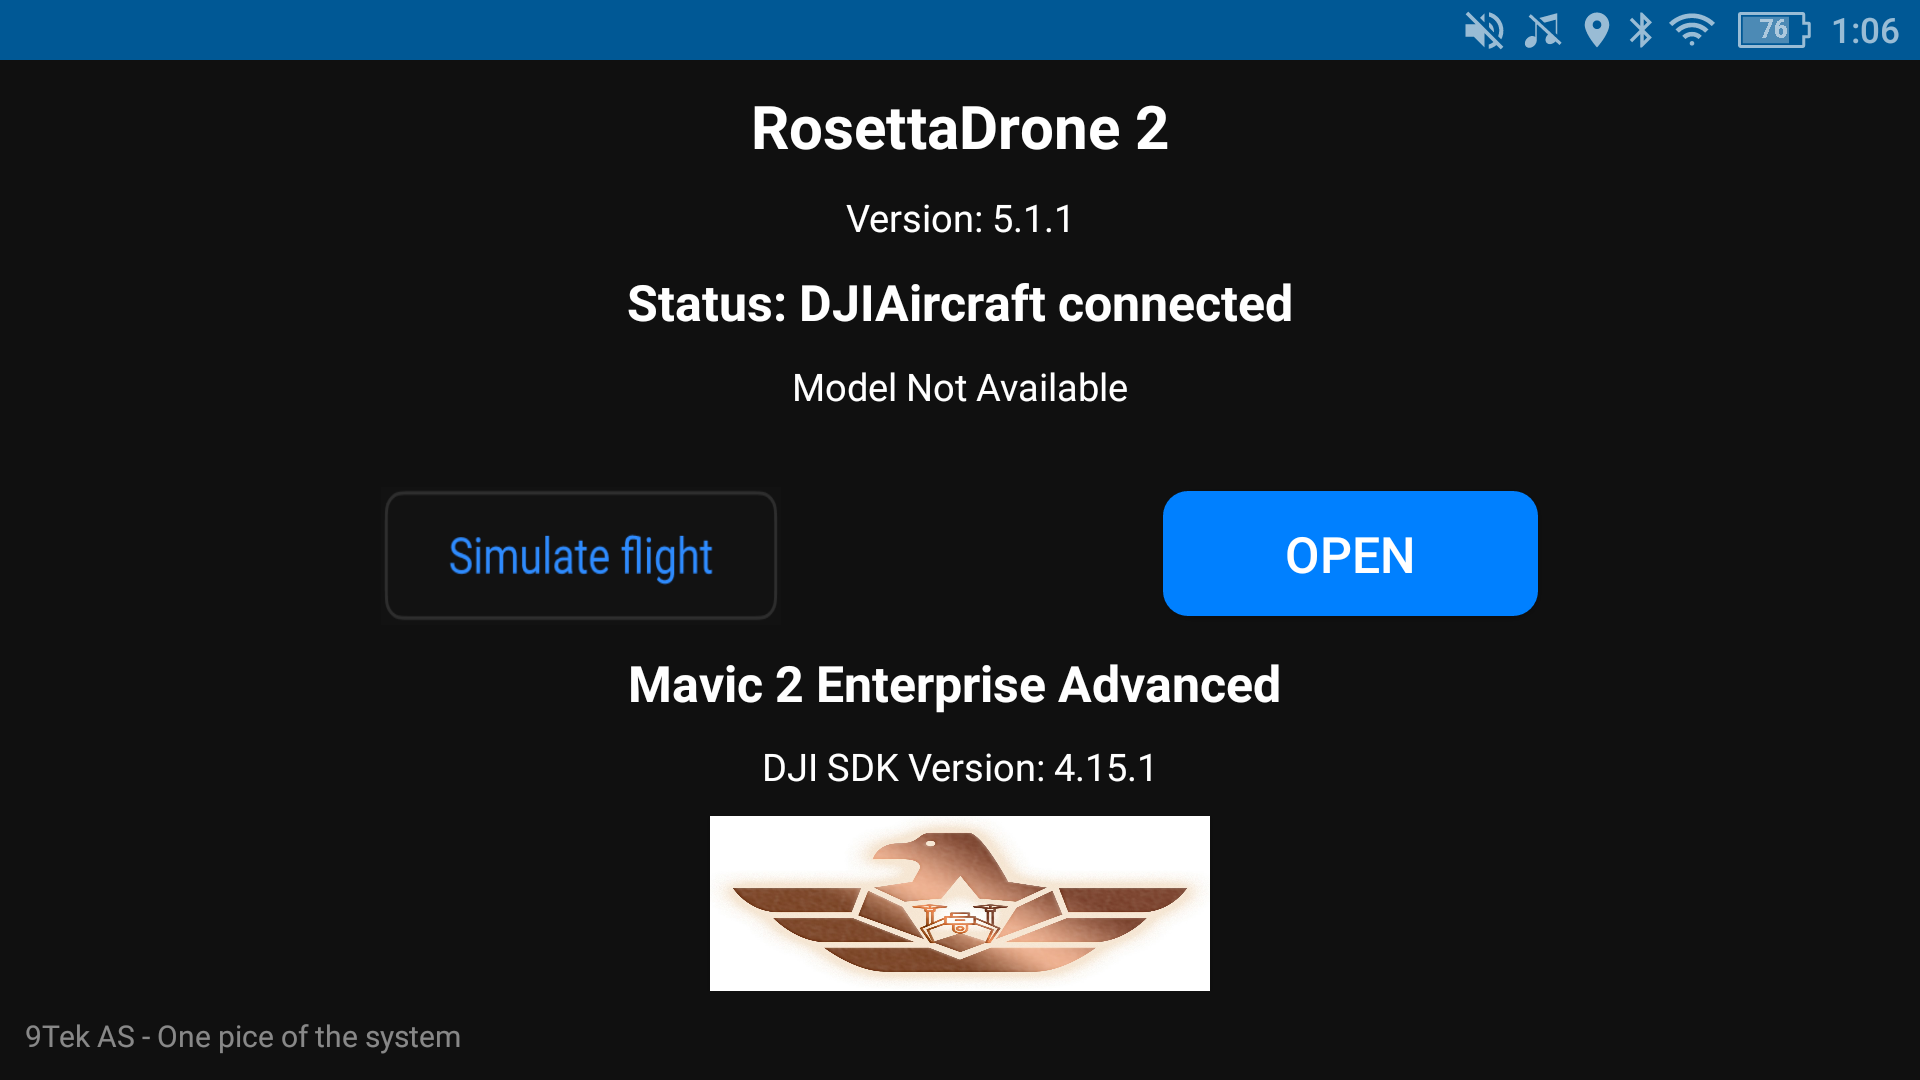
\includegraphics[width=0.8\linewidth]{./Figure/APP_Register_Page.png}
    \caption{APP启动界面}\label{Fig:append_img3}
\end{figure}

带屏遥控器APP主界面:

\begin{figure}[H]
  \centering
  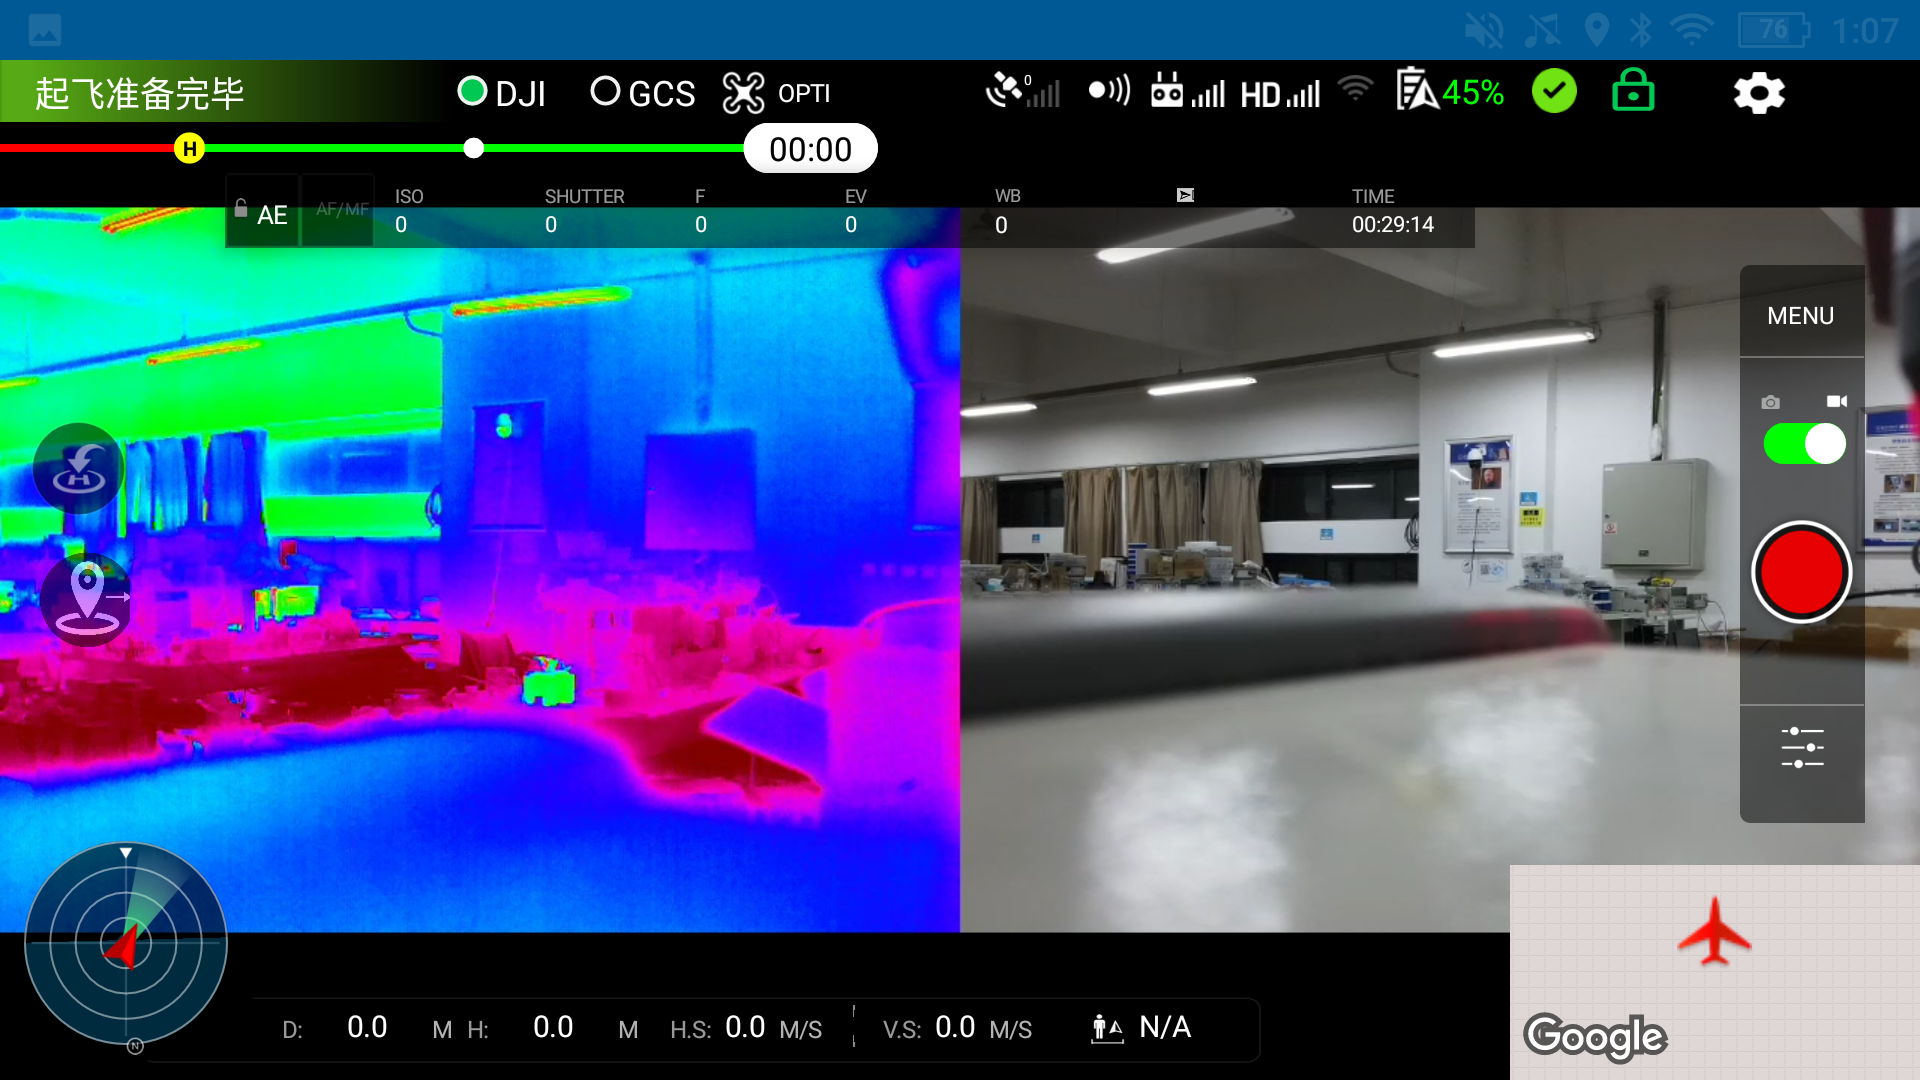
\includegraphics[width=0.8\linewidth]{./Figure/APP_Main_Page.png}
  \caption{APP主界面}\label{Fig:append_img4}
\end{figure}

带屏遥控器端QGC本机回环测试:

\begin{figure}[ht]
  \centering
  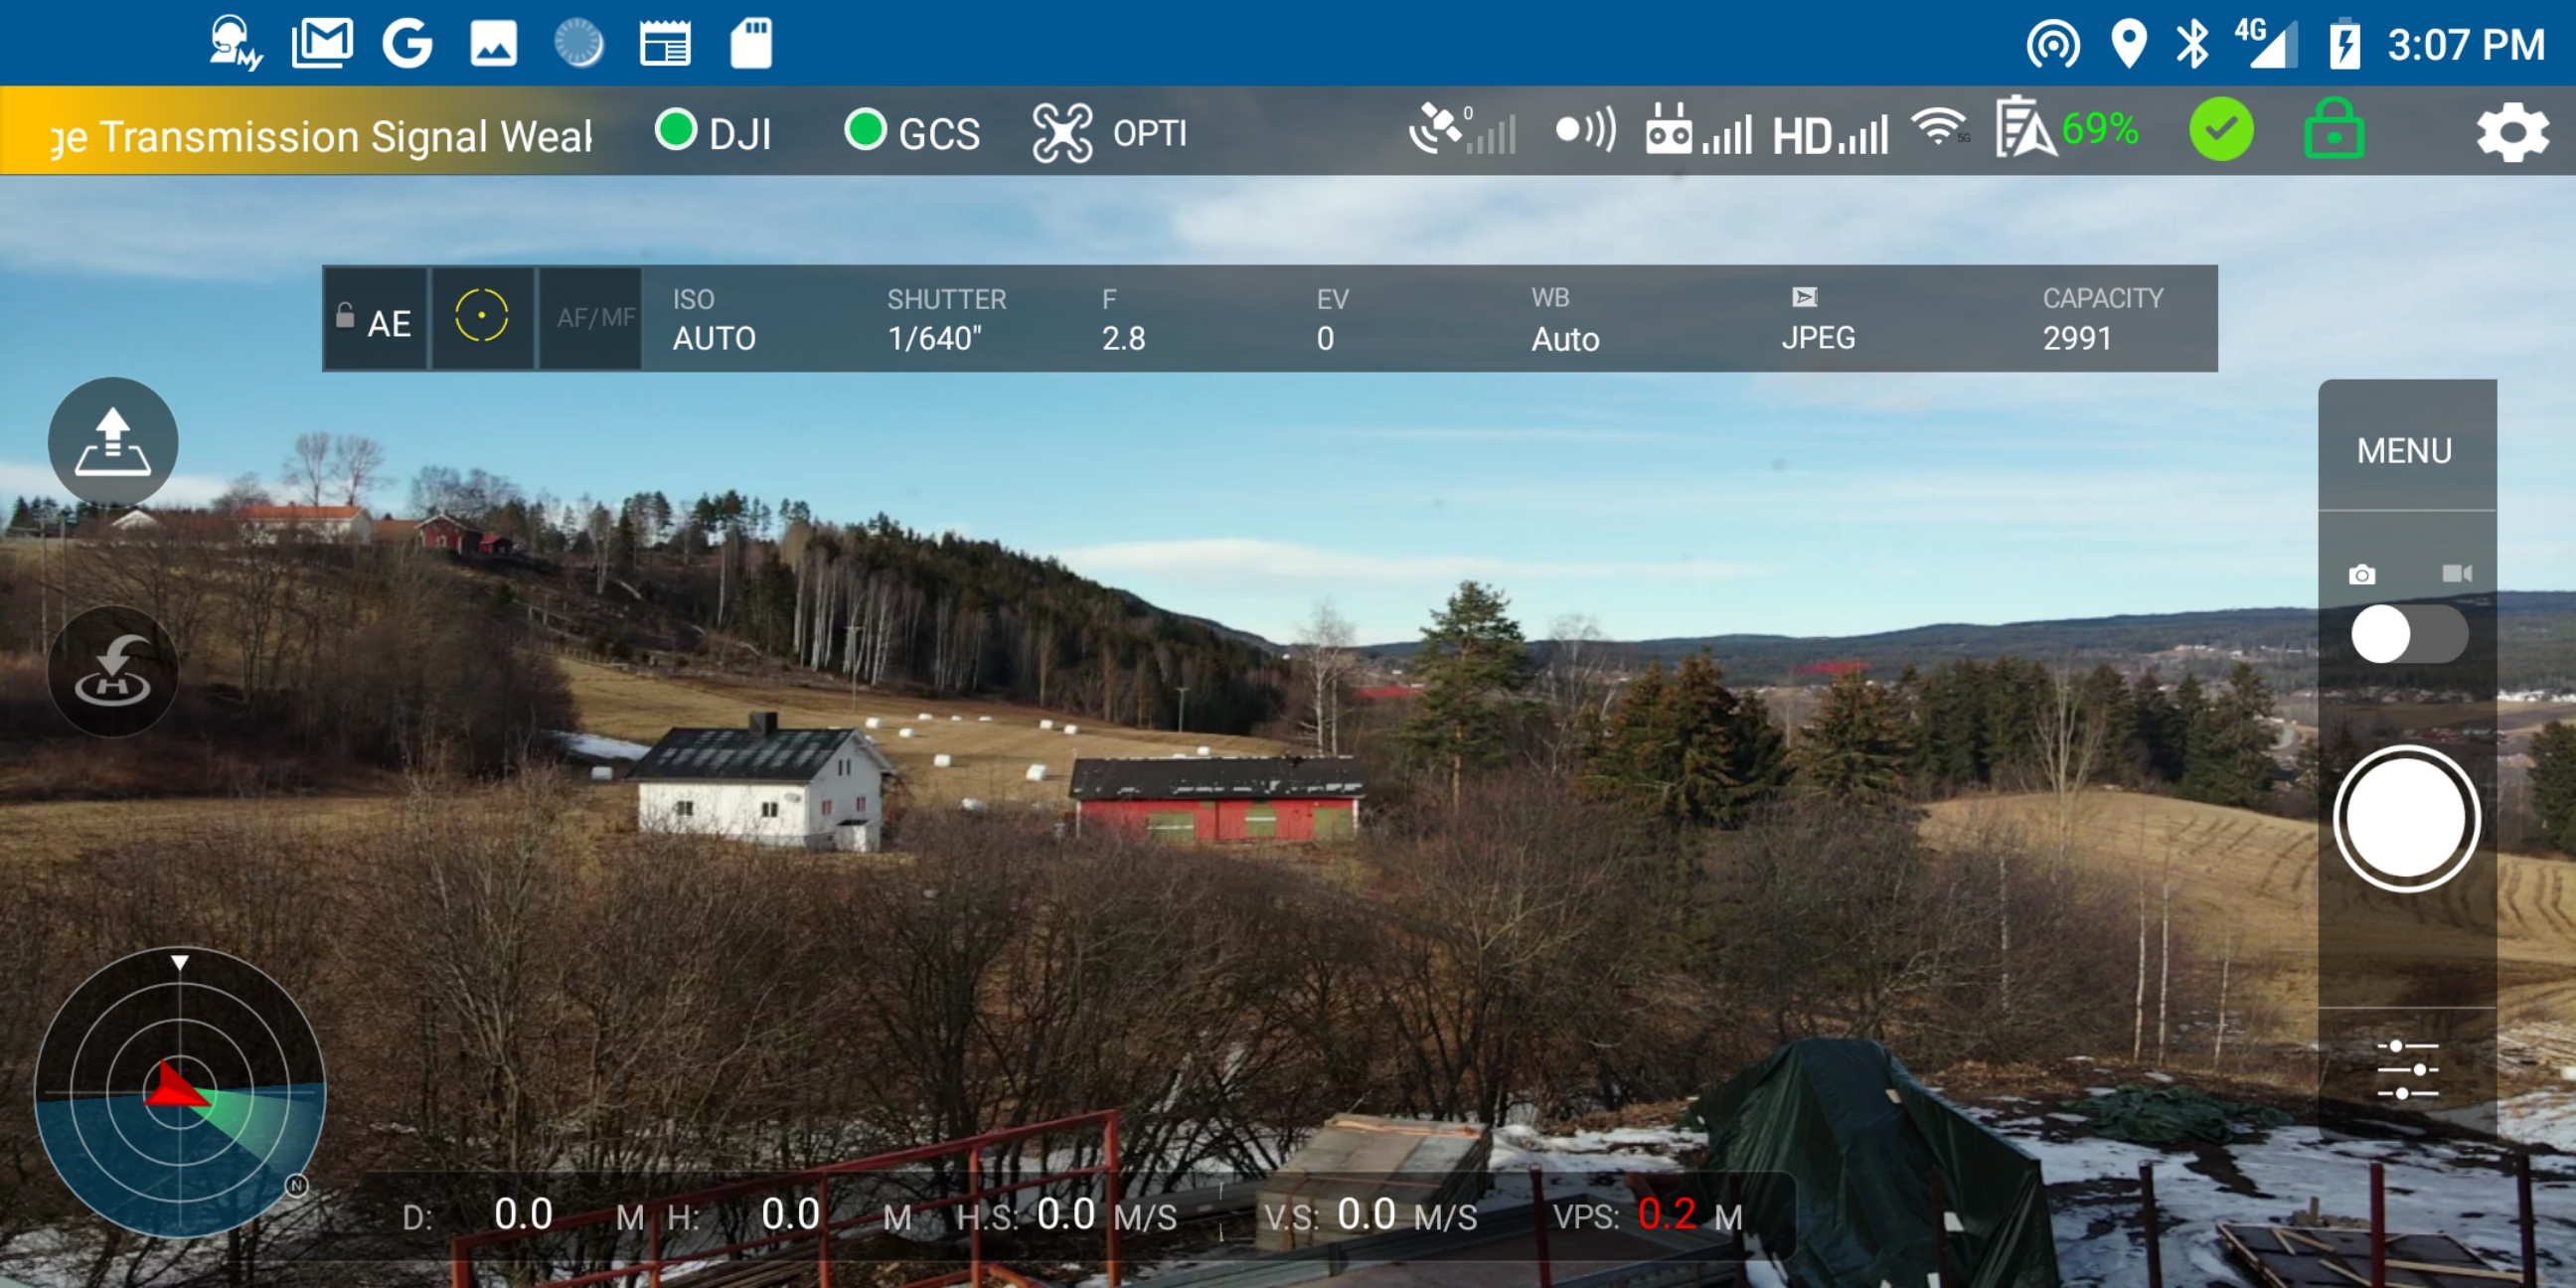
\includegraphics[width=0.8\linewidth]{./Figure/QGC_Controller_Main_Page.png}
  \caption{带屏遥控器端QGC}\label{Fig:append_img5}
\end{figure}

\section{效果测试}

第一次测试航点飞行路径:
\begin{figure}[H]
    \centering
    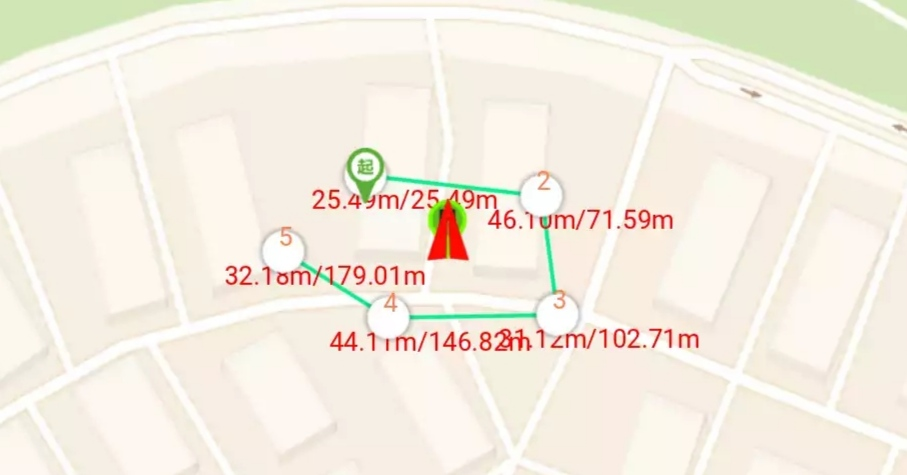
\includegraphics[width=0.8\linewidth]{./Figure/Waypoint_Flight_Test1.jpg}
    \caption{第一次测试航点}\label{Fig:append_img6}
\end{figure}

第二次测试航点飞行路径:
\begin{figure}[H]
    \centering
    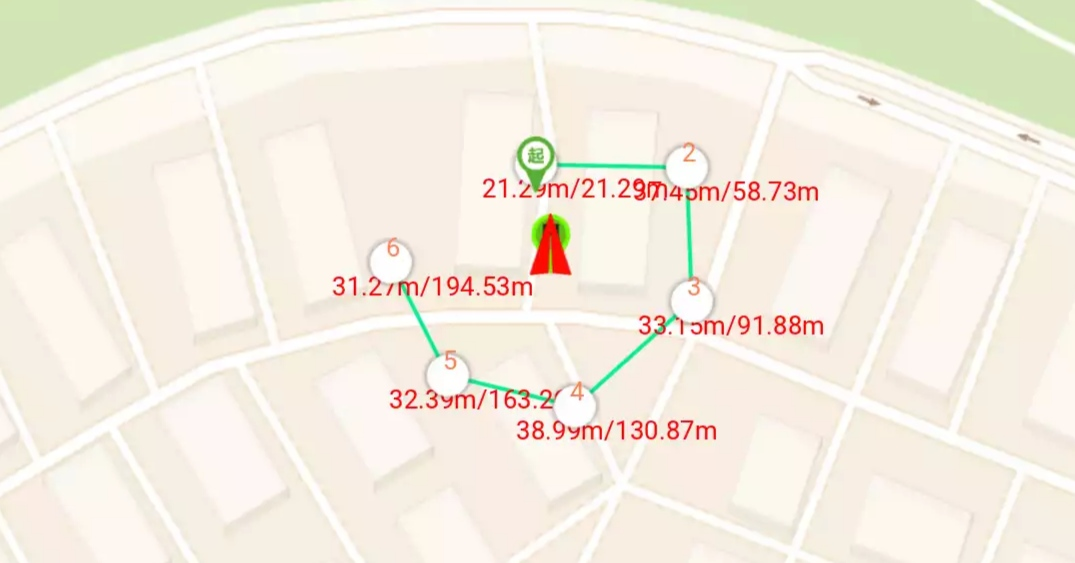
\includegraphics[width=0.8\linewidth]{./Figure/Waypoint_Flight_Test2.jpg}
    \caption{第二次测试航点}\label{Fig:append_img7}
\end{figure}

\section{控制效果}

视觉引导降落过程中,使用MPC控制算法,Pitch和Roll的角度和角速度曲线:
\begin{figure}[H]
    \centering
    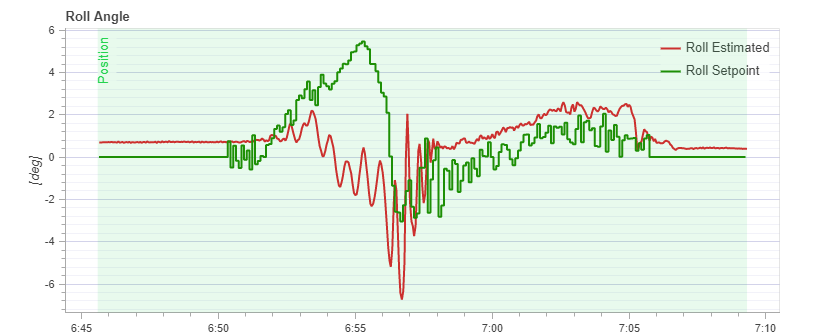
\includegraphics[width=0.8\linewidth]{./Figure/Roll_Angle_Plot.png}
    \caption{Roll角度曲线}\label{Fig:append_img8}
\end{figure}

\begin{figure}[H]
    \centering
    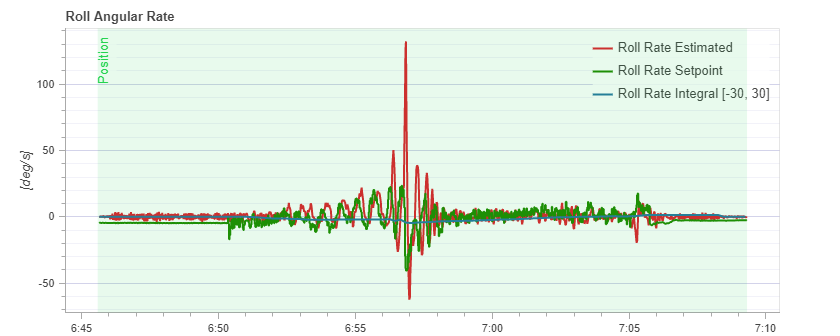
\includegraphics[width=0.8\linewidth]{./Figure/Roll_Angular_Plot.png}
    \caption{Roll角速度曲线}\label{Fig:append_img9}
\end{figure}

\begin{figure}[H]
    \centering
    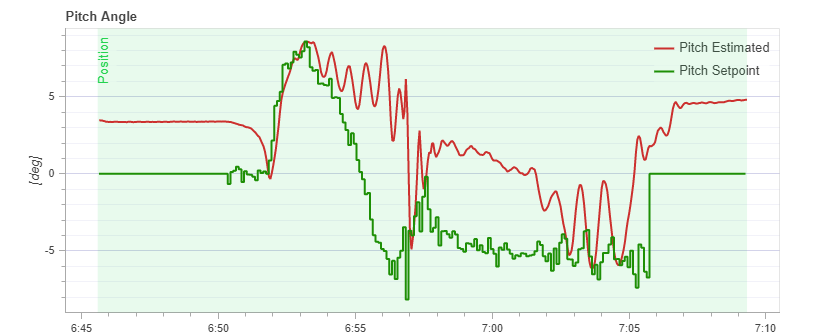
\includegraphics[width=0.8\linewidth]{./Figure/Pitch_Angle_Plot.png}
    \caption{Pitch角度曲线}\label{Fig:append_img10}
\end{figure}

\begin{figure}[H]
    \centering
    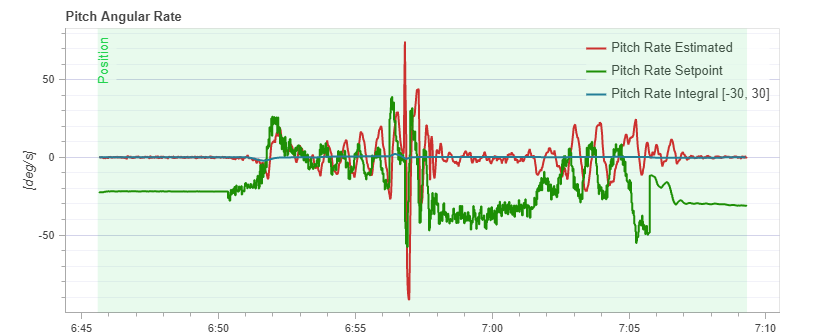
\includegraphics[width=0.8\linewidth]{./Figure/Pitch_Angular_Plot.png}
    \caption{Pitch角速度曲线}\label{Fig:append_img11}
\end{figure}

\chapter{数据}

\section{代码}
\lstinputlisting[language=Java,caption={OpenCV目标检测核心代码},label=cpp]{./Code/TargetDetect.java}
%标题不编号
\lstinputlisting[language=Java,title={OpenCV Kalman滤波器实现},label=java]{./Code/Kalman_Predict.java}
%标题不编号
\lstinputlisting[language=Java,title={原版PID控制核心代码},label=java]{./Code/VisualLandingFlightControl.java}
%无行号
\lstinputlisting[language=Matlab,title={MPC控制MATLAB仿真代码},label=matlab]{./Code/MPC_Control.m}
